
\documentclass[conference]{IEEEtran}

\usepackage{graphicx}
\graphicspath{ {images/} }

\ifCLASSINFOpdf

\else
 
\fi


\hyphenation{op-tical net-works semi-conduc-tor}


\begin{document}

\title{Project 3: A Faster IDIOT}


\author{\IEEEauthorblockN{Alex Burkhart, Nathaniel Begley, John Reynolds}}


\maketitle

% As a general rule, do not put math, special symbols or citations
% in the abstract
\begin{abstract}
The aim of this project was to take a hardware description for a processor and modify it to allow for pipelining. This will make the provided processor be much faster than it would have been prior to the modifications. Many aspects were carried over from the previous processor assignment. The original processor that was modified could have been one built by one of the team members, or the instructor provided one. The team decided to take some parts from each to make it as good as possible. The AIK specification is nearly identical to the previous one. A diagram was provided that would give a rough guideline for what was needed, and it is included later on. A top down design was created based off of this and it was used as a guide for the actual code writing. For testing, a provided Coverage tool was used to test for 100\% line coverage.  A test plan had to be created from scratch to test the newly designed processor. The processor uses 16 bit words, has 18 instructions, and will include floating point operations in the future.
\end{abstract}
% no keywords




% For peer review papers, you can put extra information on the cover
% page as needed:
% \ifCLASSOPTIONpeerreview
% \begin{center} \bfseries EDICS Category: 3-BBND \end{center}
% \fi
%
% For peerreview papers, this IEEEtran command inserts a page break and
% creates the second title. It will be ignored for other modes.
\IEEEpeerreviewmaketitle



\section{Implementor's Notes}

\subsection{Assembler Specification}
The following will outline the assembler specification for our processor design. 
Each instruction is loaded into 16 bits total with the op-code in the first 4 bits and one or two registers specified in the next 12 bits (6 bits per register).
The the op-codes for instructions and a brief explanation for each is as follows:
\begin{enumerate}
\item SYS  - Operating system call - Halts processor 
\item JZ   - Jump if zero to address in specified register
\item SZ   - Skip next instruction if value is zero
\item ADD  - Add values located in specified registers
\item AND  - Bitwise and values located in specified registers
\item ANY  - Bitwise any value located in specified register
\item OR   - Bitwise or values located in specified registers
\item SHR  - Bitshift right the value located in the specified register by 1
\item XOR  - Bitwise xor values located in specified registers
\item DUP  - Copy the value located in a register to another register
\item LD   - Load data from RAM to the register file
\item ST   - Store data from the register file in RAM
\item LI   - Load an immediate value into a reg
\item ADDF - Add 2 floating point values located in the specified registers
\item F2I  - Convert a float to an integer
\item I2F  - Convert an integer to a float
\item INVF - Compute the inverse floating point number
\item MULF - Floating point multiply
\end{enumerate}

For the purposes of this project, the floating point operations are not implemented.
Any floating point instruction will be encoded as SYS, halting the processor.
The complete assembler specification for this project is given below in Figure \ref{fig:assemblerSpec}.

\begin{figure}
	\caption{Assembler Specification}
	\centering
	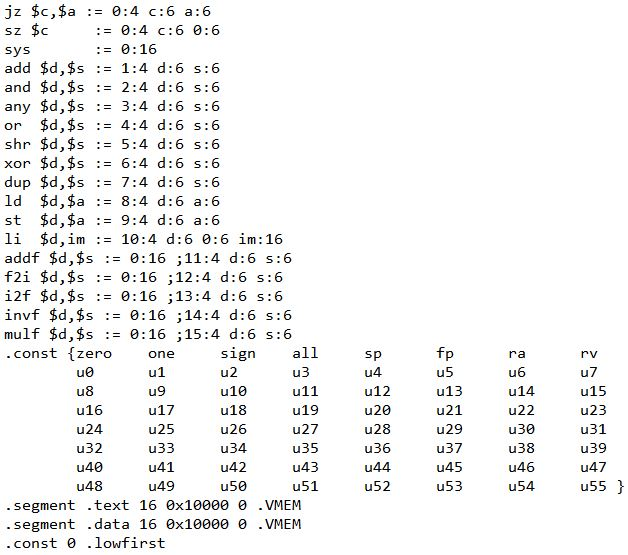
\includegraphics[width = 9cm, height=15cm,keepaspectratio]{assembler.png}
	\label{fig:assemblerSpec}
\end{figure}

It can be seen that the first three instructions are encoded similarly (as in the op-codes are the same.
The reasoning for this approach can be found in a later section.


\subsection{Design Process}
The hardware was built for the instructions that would use the ALU first. It was designed this way for future testing. This approach allowed for the testing of the most instructions before other hardware and logic needed to be added. That way, if there was an issue present, it could be solved before more complicated instructions were added in. 

Next, the hardware and control logic for the all other instructions except JZ and SZ were added. The control logic was added for each instruction and tested before moving to the next one. This was done so the error could be traced back to a specific instruction rather than a large group. 

After all of the others were functioning, SZ was added. SZ was chosen because it had the simplest implementation. It only had to make HiZ propagate through the remaining stages. Next came JZ. It was more complex than the SZ instruction. Some of the hardware and control logic designed for SZ could be used in here, so it turned out to be not as difficult as previously thought. 

The logic for the dependencies was added last, because they are unnecessary for the rest of the processor to be tested. If there was an issue here, it was important to know that it was in fact here, and not an issue with the processor itself.

\subsection{Simple Pipeline Design}
The pipeline is broken up into four stages.  The first stage makes up the instruction fetch and incrementation of the program counter.  The second stage involves reading the registers.  Stage three encompasses all of the ALU and Memory operations which contains the squashing of instructions for the implementation of the sz, jz, and li operations.  And finally, the fourth and final stage contains the writing to the registers.

The four-stage pipeline design was handled by using three 6-bit registers where each of the 6 bits can contain a word.  One of these registers was created for the first, second, and third stages of the pipeline in order to keep track of the instruction information for each of the stages and continue to pass along this information.


\subsection{Implementation Decisions}
The diagram for the created processor can be found above in Figure \ref{fig:procDiagram}.
\begin{figure}
  \caption{Processor Diagram}
  \centering
    \includegraphics[width = 9cm, height=15cm,keepaspectratio]{myproc.png}
  \label{fig:procDiagram}
\end{figure}

%\includegraphics{myproc.png} 
The state machine which controls the processor consists of 23 states which are responsible for directing the execution of all instructions.
For one word instructions (all but LI), the controller loads the instruction into the instruction register and then executes the instruction.
If the instruction is two words long, the state machine recognizes the two-word instruction op-code from the first instruction fetch and loads the second word into the MDR. 
Since the only two word instruction is LI, there will be no conflicting states between two word instructions.
In order to fit 18 instructions into a bit field of size 4, the instructions JZ, SZ, and SYS were consolidated to a single path in the state diagram.
This was done because these three instructions perform a similar function (not to mention the assignment specified combining these specific instructions).


This section will discuss the various reasons for the architecture, design, and implementation decisions.

The first design hurdle was to eliminate the sz instruction in order to keep the number of instructions at 16 and maintain a bit field size of 4.  This decision was simple since the same functionality can be accomplished by simply using the jz instruction.  Additionally, this takes off some additional programming burden of implementing the squashing for the sz instruction.  The sys instruction is also bundled here due to it's similar functionality.

Another obstacle was how to handle the instructions which may not necessarily use the +1 incrementation of the program counter.  The jz instruction for example needs to jump to a specified address if the register contains a zero value.  In order to tackle this issue, we decided to go ahead and load the next instruction into the pipeline, but simply "squash", or in other words just nullify this operation, if the jump was needed.

The li instruction required some tricky programming as well. The words were grabbed on the same clock cycle. This op code would then trigger another memory read to occur. This was done to simplify how each stage would esecute for a given instruction. All instructions would now be ready for execution in the one clock cycle. This also helped simplify the previously mentioned jump and squash instructions.

The ALU used in this project was the exact one used by Alex Burkhart in the previous project. This was done because it reduced the workload for the team. This ALU had very simple inputs and outputs and could be ported over for this project with relative ease. 

For the stages, there were a couple very specific choices made by the team. Each stage was given the same size memory. This was done to make both designing and testing simpler in the future. Dependencies were handled by using simple flags. These flags would cause the affected stage to halt where it was. 


Another major decision was to not use a separate control line for each control signal.
As the number of control signals increased, it became less and less feasible to have named wires going to and from each module.
Instead, one control line of width 64 was implemented.
The control line's control signals are as follows:

\begin{itemize}
\item controls[0] = irin;
\item controls[1] = irout;
\item controls[2] = pcin;
\item controls[3] = pcout;
\item controls[4] = mdrin;
\item controls[5] = mdrout;
\item controls[6] = marin;
\item controls[7] = marout;
\item controls[8] = yin;
\item controls[9] = yout;
\item controls[10] = zin;
\item controls[11] = zout;
\item controls[12] = regin;
\item controls[13] = regout;
\item controls[14:19] = selreg;
\item controls[20] = memread;
\item controls[21] = memwrite;
\item controls[22] = outputenable;
\item controls[23:26] = aluop;
\item controls[27] = mfc;
\item controls[28:63] = X (not used);
\end{itemize}
The controls line is of the type [0:63] instead of [63:0].
This was done for no reason other than to try it.

Each register used will output its current value or HiZ on the rising edge of every clock cycle.
Also, each register will latch values from the bus on the falling edge of every clock cycle.
This was implemented using two always blocks for both ends of a clock cycle. 
The reason for doing this was to limit the already large number of clock cycles this multi-cycle machine will take to execute a program.

A Von Neumann architecture was selected because it seemed easier to implement.
The only "difficulty" would be making sure the RAM is partitioned for instruction memory and data memory.
This "difficulty" is overcome by specifying how the RAM gets set during simulation.
AIK will output the RAM file in exactly the way it needs to be for the machine.


\subsection{Test Bench Decisions, Methods, and Coverage}
Everything was tested sequentially. So each instruction was tested as it was designed. This was done so that if an error was found, we knew exactly where it was and could fix it quickly. After this was all tested, a simple test bench was made that only checked to see if multiple instructions could be executed. Dependencies were not added yet. After dependencies were added, small programs of roughly 3 instructions were used for testing. After all of the small tests were done, a full test bench was created to check all lines and states to verify that they worked correctly. 

The test bench developed does several things. 
It checks the validity of each instruction (whether or not the instruction did what it was supposed to do) and it has a good coverage of testing. 
Using the coverage analyzer, the test bench developed has 100\% line coverage and 100\% finite state machine coverage. 
This means that the test bench covers each state and every path to and from each state. 
It also touches every single line of code, meaning there are no untested, nor unused, lines of code in the project.
After testing, the outputs from the register file and RAM are compared to what the actual expected values are.
For this project and test, the values all matched.
To determine whether or not the program passed, for every error a \$display will show what the specific error was.

Note that for running this project, the entirety of our RAM is compressed to a single 65536*16 bit wire, which increases the execution time substantially.
If the program looks like it freezes, just wait and it will eventually finish.


\subsection{Issues}
There are no known bugs or issues present in the submitted code.
% You must have at least 2 lines in the paragraph with the drop letter
% (should never be an issue)

\hfill P3
 
\hfill 04/18/2016



\end{document}

